
% To train a generalizable world action model, we first require a video model that can generalize across diverse manipulation tasks while supporting real-time inference. However, existing video foundation models are ill-suited for this purpose. First, they are primarily designed for content creation and therefore prioritize aesthetic quality over fine-grained manipulation dynamics. Second, they typically operate at high spatial and temporal resolutions to maximize visual fidelity, resulting in computational costs incompatible with real-time policy inference. 
\vspace{-1mm}
\section{Data Processing Pipeline}
\vspace{-1mm}
In this section, we describe our data collection and curation pipeline, including how we unify the inputs and outputs across diverse manipulation datasets.

\textbf{Video Sources.}
We compile a large-scale, diverse collection of manipulation videos for continued pretraining of an open-source video foundation model~\citep{wan2025wan}. Our data span three categories: robot manipulation datasets, human activity datasets, and general-purpose video datasets. For general-purpose video datasets, we apply an extensive filtering pipeline similar to that of LVP~\citep{chen2025large} to retain only videos depicting manipulation-related activities. Table~\ref{table:video_source} summarizes the datasets used for training; full dataset references are provided in Appendix~\ref{app_data}.

\begin{table}[h]
    \centering
    \small
    \setlength{\tabcolsep}{4pt}
    \renewcommand{\arraystretch}{1}
    \begin{tabularx}{\linewidth}{@{}llX@{}}
        \toprule
        Data Type & Embodiment Type & Data Sources \\
        \midrule
        \multirow{3}{*}{Robot}
        & Single-arm
        & OXE, RoboMIND, DROID, RH20T, MolmoAct \\
        & Dual-arm
        & AgiBot World-Beta, RoboCOIN, RDT, GM-100, ABC-130K, Self-collected ALOHA Data\\
        & Mobile \& humanoid
        & InternData-A1, Galaxea Open-World, Self-collected dexterous hands \\
        \midrule
        \multirow{2}{*}{Human}
        & \multirow{2}{*}{Human hands}
        & Open-source: EgoDex, Ego4D, EPIC-KITCHENS, Something-Something V2, VITRA-1M \\
        & & Self-collected egocentric data\\
        \midrule
        General Video
        & Human hands
        & OpenVid, Panda-70M \\
        \bottomrule
    \end{tabularx}
    \caption{Overview of training data sources. Full dataset references are provided in Appendix~\ref{app_data}, Table~\ref{table:video_source_full}.}
    \label{table:video_source}
    \vspace{-3mm}
\end{table}

\textbf{Video Filtering, Segmentation and Captioning.}
We first remove corrupted trajectories, including those with camera failures or abrupt discontinuities, and segment the remaining trajectories into semantically coherent clips lasting 1--12 seconds. We identify candidate boundaries using heuristic cues associated with natural transitions, such as local minima in human-hand or end-effector velocity and moments when the gripper or fingers open or close. A vision-language model (VLM) then refines the segmentation by merging adjacent clips where appropriate and adjusting their start and end points.

After segmentation, we generate detailed captions that describe the task, explicitly identify the active end effectors, unambiguously specify the target objects, and characterize the camera views and motion. Figure~\ref{fig:fig2} illustrates an example, and Appendix~\ref{app_video} provides further details.




\begin{figure}[t]
    \centering
    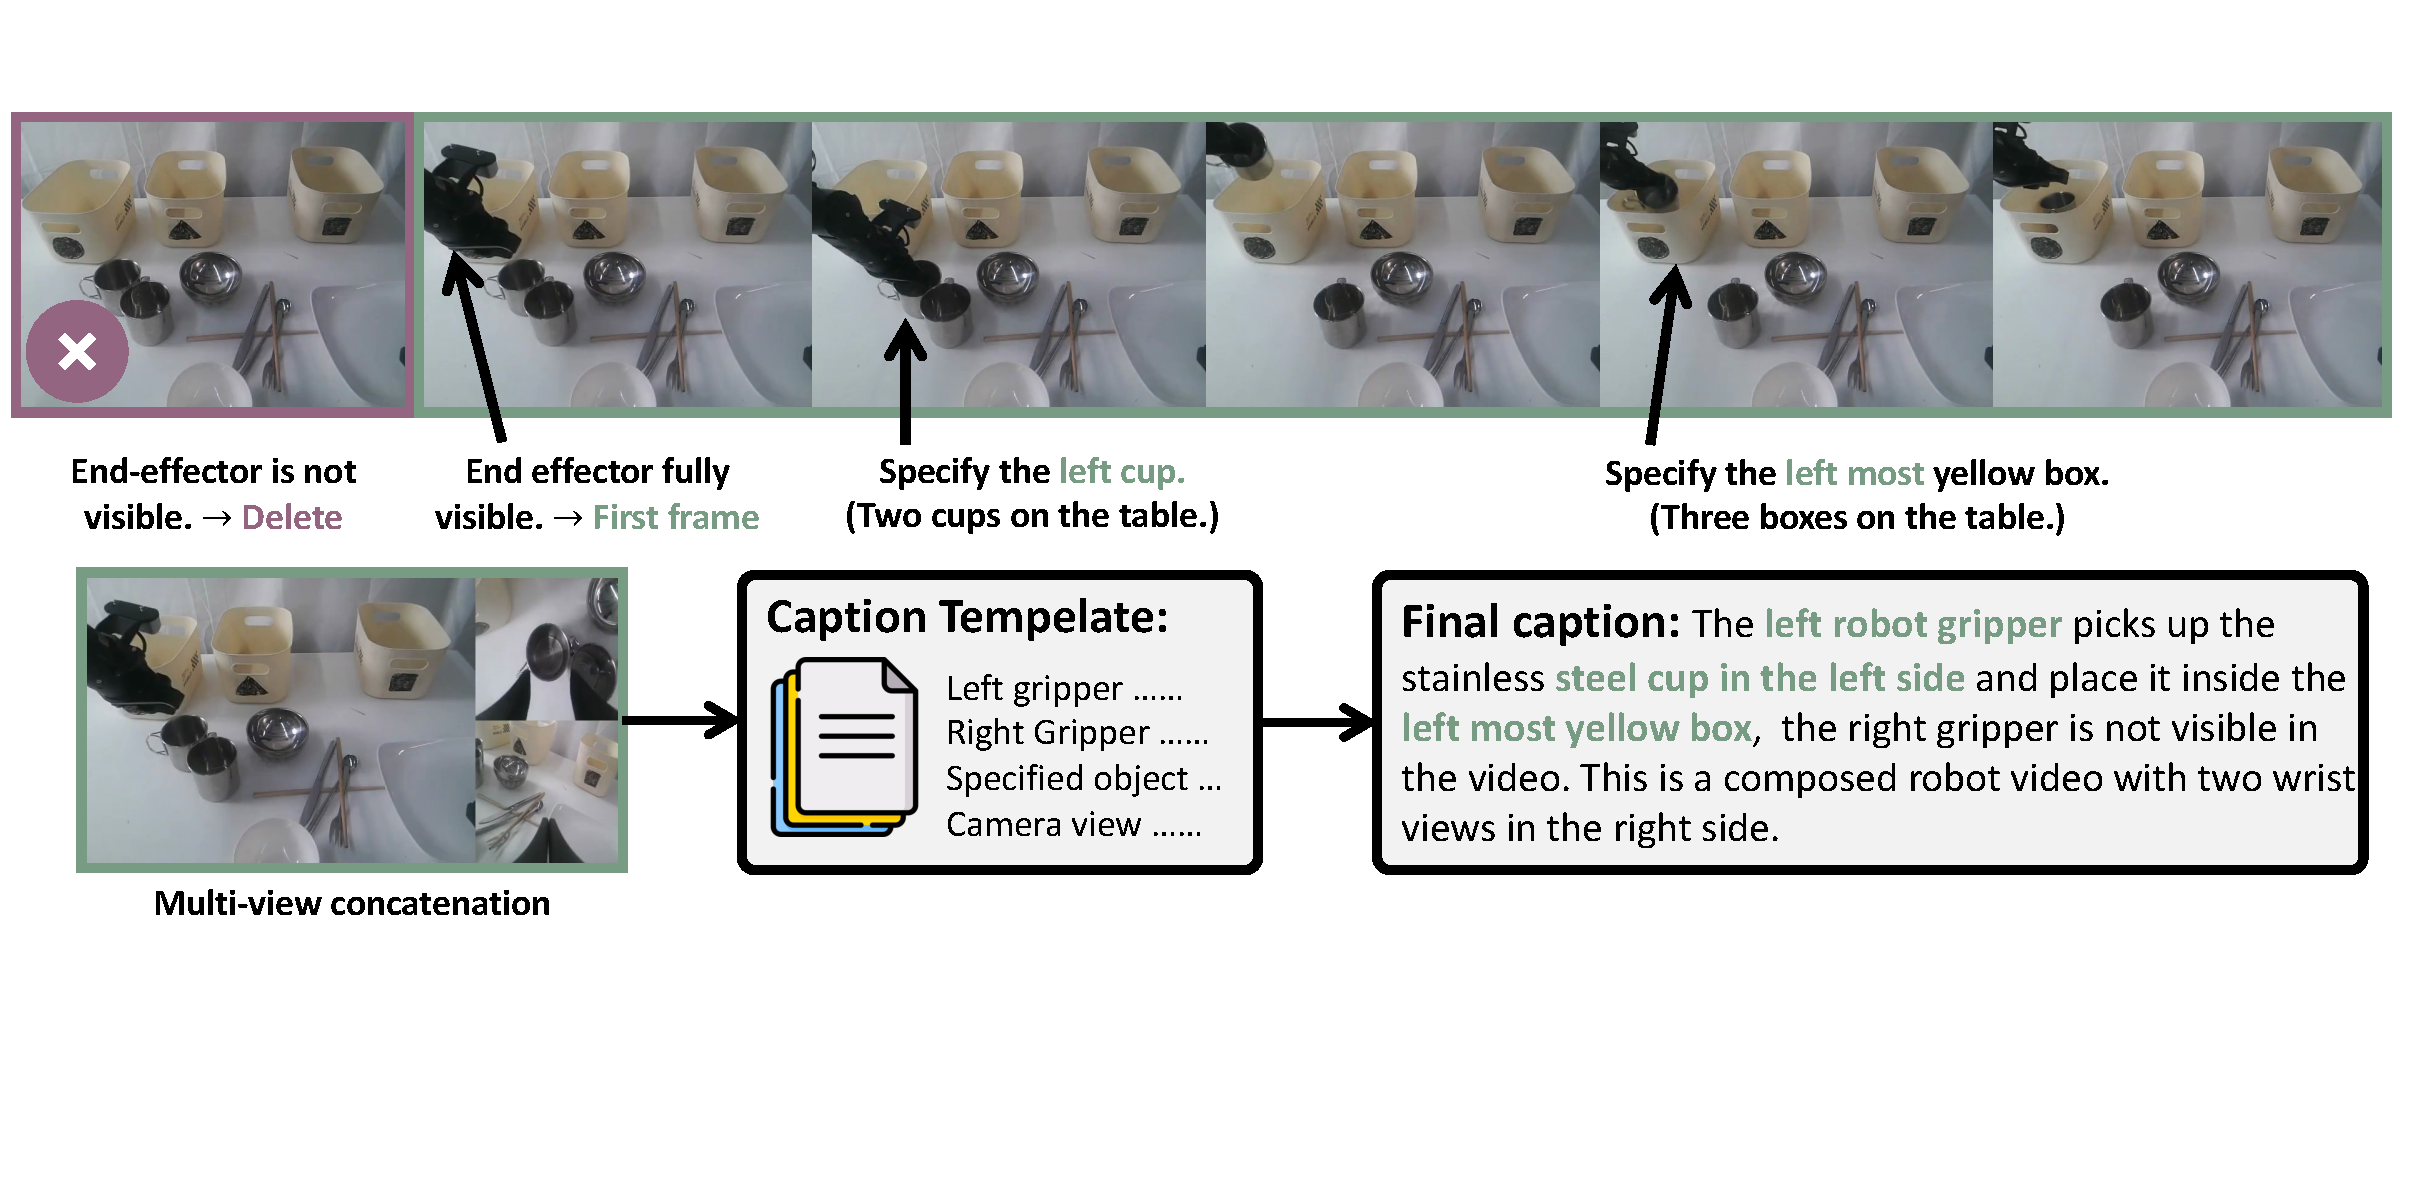
\includegraphics[width=0.85\linewidth]{figures/fig2_2.pdf}
    \caption{An example of our data processing pipeline. The central objective is to reduce uncertainty in future prediction, thereby encouraging the model to learn a consistent mapping from conditioning information to sub-task trajectories. To this end, each caption includes detailed task descriptions, explicit end-effector identification, a description of the visible target object, and camera-view changes.}
    \label{fig:fig2}
    \vspace{-4mm}
\end{figure}





\begin{wrapfigure}{t}{0.48\textwidth}
    \vspace{-12pt}
    \centering
    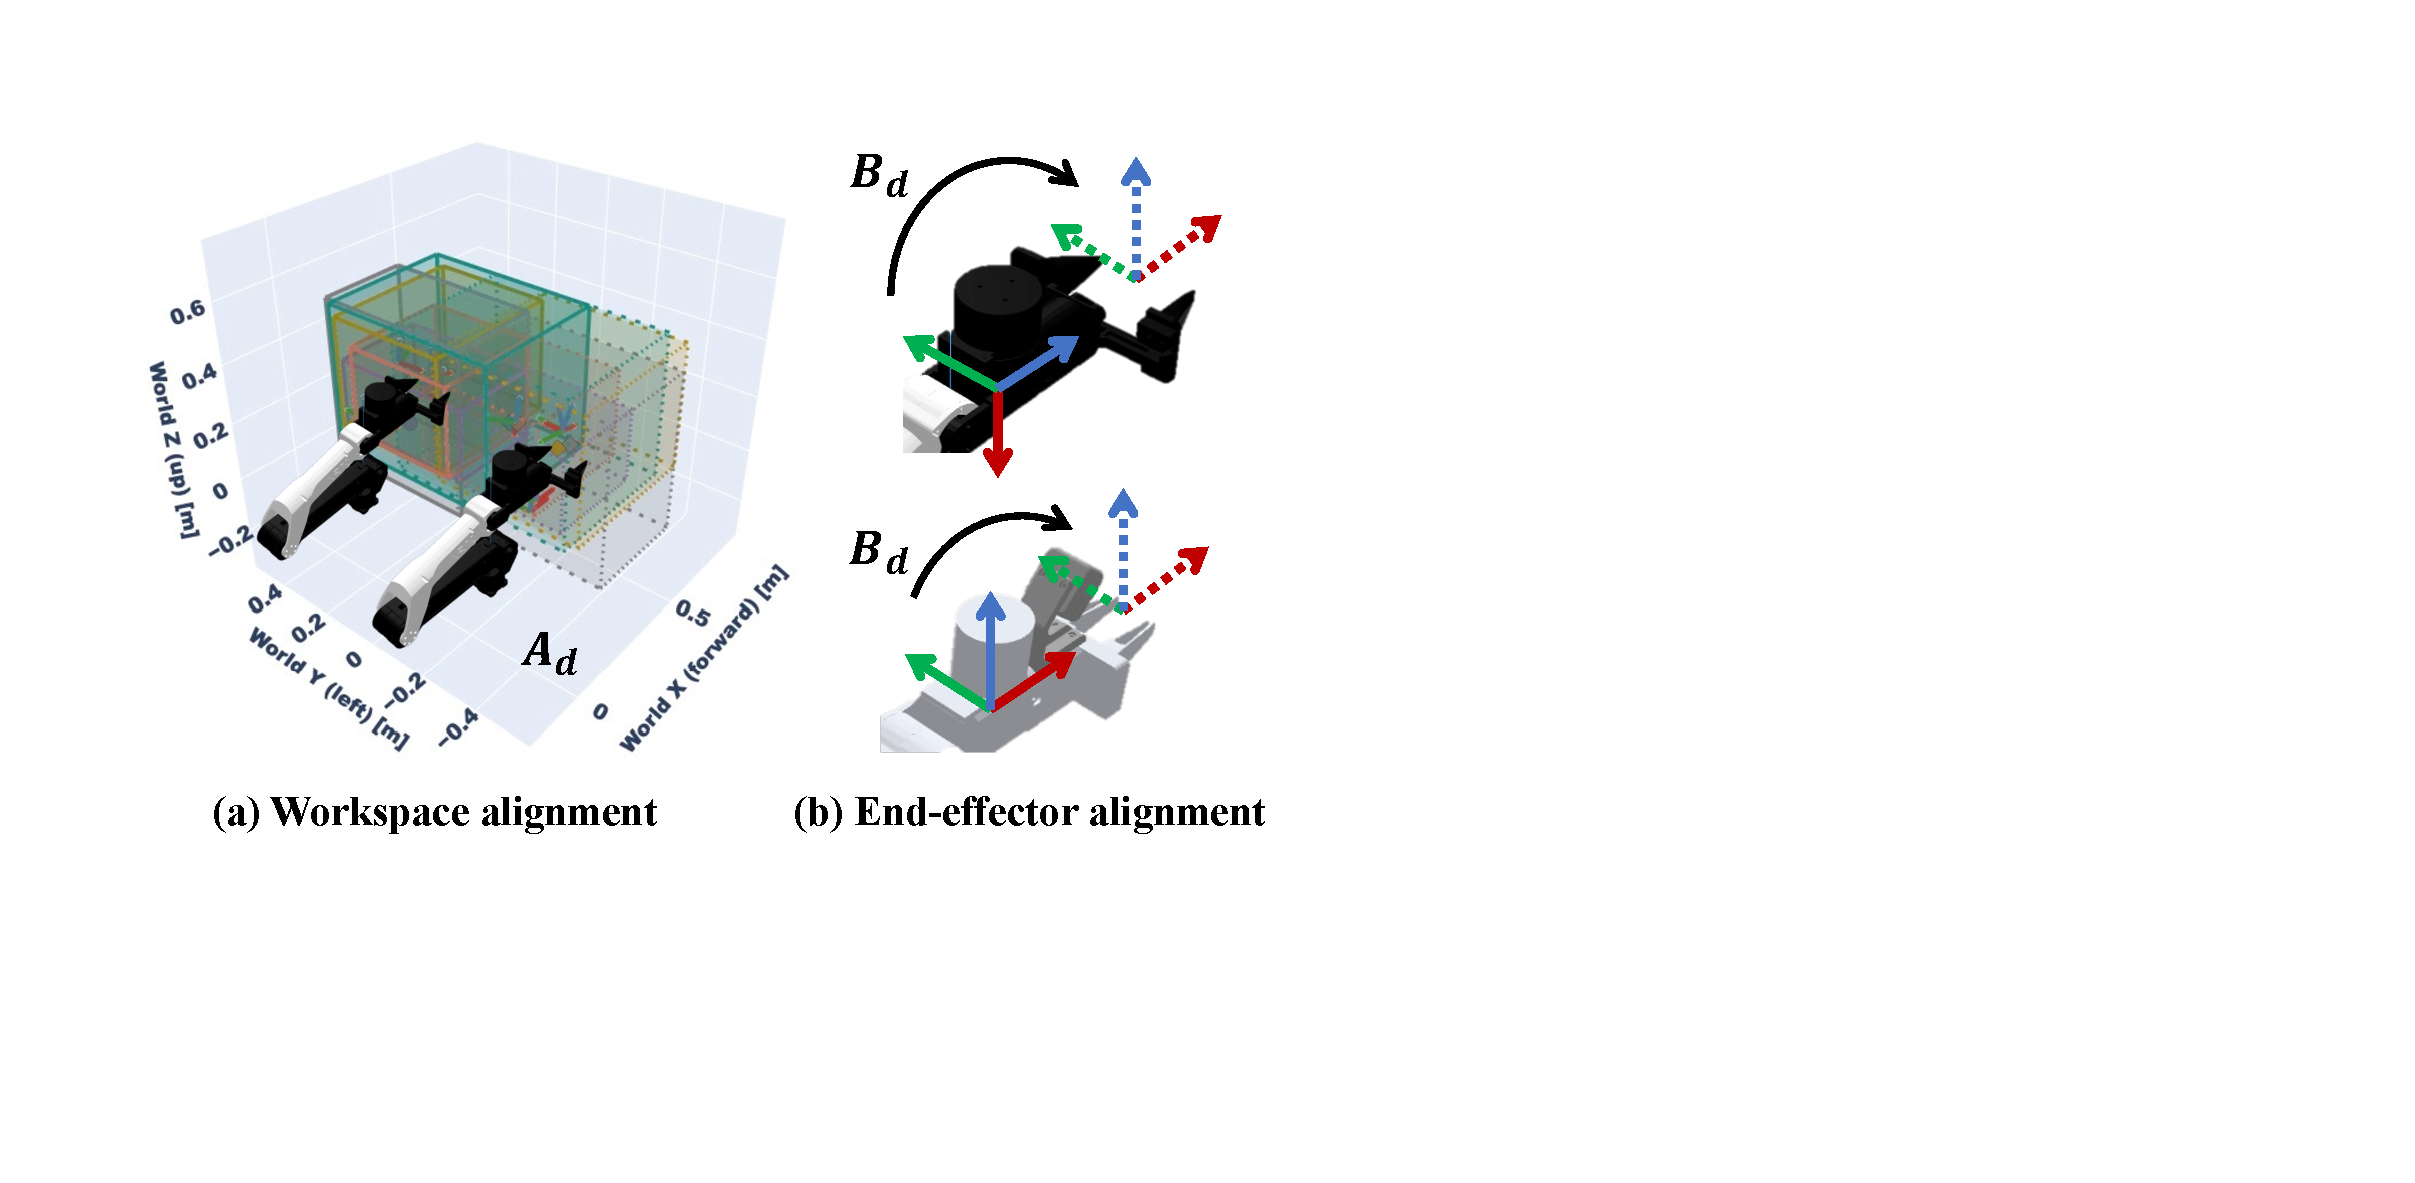
\includegraphics[width=\linewidth]{figures/fig3_2.pdf}
    \caption{(a) Bounding boxes show the aligned workspaces of different datasets. (b) Aligned end-effector coordinate frames.}
    \label{fig:coordinate_alignment}
    \vspace{-12pt}
\end{wrapfigure}


\textbf{Unified Action Space and Unified End-effector Coordinate Systems.}\label{data:action}
Different robot datasets often adopt inconsistent coordinate systems and camera viewpoints, resulting in conflicting action representations for visually similar motions. For example, a leftward motion may correspond to the positive \(x\)-direction in one dataset but the negative \(y\)-direction in another, making it difficult for the model to learn the semantic meaning of each action dimension.

We focus on egocentric bimanual datasets, including ALOHA-style,
humanoid-style, and human egocentric datasets. These datasets
account for more than \(80\%\) of the total data and share a
similar bimanual structure and camera viewpoint.
We explicitly align their coordinate systems at two levels:
(1) \textit{workspace alignment}, which applies a world-frame
transformation so that different robots have comparable
end-effector workspaces; and (2) \textit{end-effector alignment},
which applies a local transformation to standardize end-effector
origins and axis orientations. 

% Such alignment is necessary because different datasets adopt different end-effector conventions. For example, some place the eef origin between the fingertips, whereas others place it at the gripper mounting link. Similarly, some align the \(x\)-axis with the gripper direction, while others define it perpendicular to that direction.

For an arm dataset \(d\) , let
\(T_d = {}^{W_d}T_{E_d} \in SE(3)\) denote the original
end-effector pose, where \(W_d\) and \(E_d\) are the dataset's
world and end-effector frames, respectively.
We define the workspace alignment as
\(A_d = {}^{\bar{W}}T_{W_d}\) and the end-effector alignment as
\(B_d = {}^{E_d}T_{\bar{E}}\), where \(\bar{W}\) and \(\bar{E}\)
denote the canonical world and end-effector frames.
The aligned end-effector pose is given by $\widetilde{T}_d = A_d T_d B_d,
    \label{eq:coordinate_alignment}$.



\textbf{Unified T-shape Multi-view Input across Datasets.} 
Robotics datasets commonly contain observations from multiple camera views. We arrange them into a T-shaped composite image, with the primary view on the left and two auxiliary views stacked vertically on the right, as illustrated in the bottom-left panel of Figure~\ref{fig:fig2}. When fewer than two auxiliary views are available, we fill the missing slots with black placeholder images.

% \begin{equation}
%     \widetilde{T}_d = A_d T_d B_d,
%     \label{eq:coordinate_alignment}
% \end{equation}
% where \(A_d \in SE(3)\) aligns the world coordinate system
% through left multiplication, and \(B_d \in SE(3)\) aligns
% the end-effector origin and axis orientations through
% right multiplication.
% Such alignment is necessary because different datasets adopt
% different end-effector conventions. For example, some place
% the end-effector origin between the fingertips, whereas others
% place it at the gripper mounting link. Similarly, some align
% the \(x\)-axis with the gripper direction, while others define
% it perpendicular to that direction. The local transformation
% \(B_d\) accounts for both the origin offset and the difference
% in axis orientations.







\section{VPP2: A Generalist Policy with Zero-shot Capability}

\textbf{Overview.}
Our large-scale, diverse, and densely annotated dataset enables us to train a policy with strong generalization capabilities. VPP2 builds upon the pretrained Wan2.1-I2V-14B model~\citep{wan2025wan} and introduces an action expert via a mixture-of-transformers (MoT) architecture~\citep{liang2025mixture}. Our training objective is twofold: we first adapt the video model to produce generalizable future predictions at real-time inference speed for open-ended manipulation tasks, and then train the action expert conditioned on the KV cache of the video model. To maximize policy generalization, we organize training into the stages summarized in Figure~\ref{fig:fig4}.

% \begin{table}[h]
%     \centering
%     \small
%     \setlength{\tabcolsep}{4pt}
%     \renewcommand{\arraystretch}{1.15}
%     \begin{tabularx}{\linewidth}{@{}cllX@{}}
%         \toprule
%         Stage & Training Type & Prediction Target & Dataset \\
%         \midrule
%         1 & Video Continue Pre-training
%           & Complete Video Event
%           & General Video, Full Manipulation Video \\
%           \midrule
%         2 & Video Post-training
%           & Long Video Chunk
%           & Full Manipulation Video \\
%           & +Video Distillation
%           & 
%           &  \\
%         \midrule
%         3 & Action Expert Pre-training
%           & Short Action Chunk
%           & Full Dual-Arm Manipulation trajectories \\
%         \bottomrule
%     \end{tabularx}
%     \caption{The VPP2 training pipeline consists of three stages. Stage 1 performs large-scale, event-level video pretraining to obtain a generalizable video model for manipulation. Stage 2 post-trains and distills the model to predict long-horizon video chunks(8 seconds) with a single forward pass in approximate 0.1 second. Finally, Stage 3 freezes the video model and trains an action expert to generate 2 seconds action chunk conditioned video latent.}
%     \label{table:training_pipeline}
% \end{table}

% \subsection{Video Prediction Model Training Pipeline}

% \textbf{Event-level Video Model Continue Pre-training.}
% In this stage, we want train a generalizable video model in manipulation domain. We noticed that state-of-the-art pretrained video model are often trained with bidirectional attention DiT architecture and prompt enhancement. Following these works, we also predict trajectories at event level, so that the subtask description have a clear mapping to the predicted trajectories. In this stage,  we directly down-sample video to desired frame numbers $N$ and always predict from starting point(t=0) to the end point with flowing matching objective:
% \[
% \mathcal{L}_{FM}
% = \mathbb{E}_{x_s,\,\epsilon,\,s}
% \left\| \hat{x}_1(x_{s}, s, c) - x_1 \right\|^2,
% \]
% where the prediction target $x_1 = \{o_{T/N},o_{2T/N},...,o_{(N-1)T/N},o_{T}\}$ is sampled uniformly from a trajectory$\tau$ with total length $T$,  
% $x_{s} = sx_1 + (1-s)\epsilon$ denotes the noised future at flow-matching step $s \in [0, 1]$ , and $c$ represents all conditioning inputs, including the language instructions and the initial observation $o_0$.

% In this stage, we continue pre-train the base model Wan2.1-I2V-14B model for 30,000 steps at batch size 1024 and learning rate 1e-5. In experiment part, we will show that our model performs significantly better than base Wan-14B model in manipulation instruction following ability. Moreover, our 14B model even have better instruction following than Cosmos3-Super-Image2Video model with 64B size.

% \textbf{Chunk-level Video Model Post-training.}
% After continue-pretraining, we get a video model that can predict at event-level and generalize well on manipulation tasks. However, this event-level video prediction can be at various manipulation speed which put burden on action learning. Therefore, we post-training it to generate a fixed length of future prediction which easy for action learning. The interval between frames becomes $\delta =fH/N$ where H is predicted video second and $f$ is the frame per second of the dataset. The prediction target $x_1$ becomes $x_1 = \{o_{\delta},o_{2\delta},...,o_{N\delta}\}$

% Finally, we do video distillation with consistency loss:


\subsection{Video Prediction Model Training Pipeline}


\textbf{Stage 1: Event-level Video Model Continued Pre-training.}
We first adapt a pretrained video generation model to the manipulation
domain through event-level continued pre-training.
Each training example covers a complete manipulation subtask, aligning
the subtask description with the corresponding visual evolution from
the initial observation to subtask completion.

Given a demonstration $\tau = (o_0, o_1, \ldots, o_T)$,
we uniformly sample $N$ future frames across the entire event:
\begin{equation}
    \mathbf{y}_{\mathrm{event}}
    =
    \left( o_0,
        o_{\lfloor T/N \rfloor},
        o_{\lfloor 2T/N \rfloor},
        \ldots,
        o_T
    \right),
\end{equation}
where $T$ is the final frame index and $N$ excludes the initial
conditioning frame $o_0$.
Let $\mathbf{x}_1 = \mathcal{E}(\mathbf{y}_{\mathrm{event}})$
denote the corresponding video latent representation, where
$\mathcal{E}$ is the video encoder.
We construct the interpolated latent as
\begin{equation}
    \mathbf{x}_s
    =
    (1-s)\boldsymbol{\epsilon} + s\mathbf{x}_1,
    \qquad
    \boldsymbol{\epsilon} \sim \mathcal{N}(\mathbf{0}, \mathbf{I}),
    \quad s \in [0,1],
\end{equation}
where $s$ denotes flow time, with $s=0$ corresponding to noise and
$s=1$ to data.
The model is optimized with the flow matching objective~\citep{lipman2023flow}
\begin{equation}
    \mathcal{L}_{\mathrm{FM}}(\theta)
    =
    \mathbb{E}_{(\mathbf{x}_1,c),\,\boldsymbol{\epsilon},\,s}
    \left[
        \left\|
            v_\theta(\mathbf{x}_s,s,c)
            -
            (\mathbf{x}_1-\boldsymbol{\epsilon})
        \right\|_2^2
    \right],
    \label{eq:video_fm}
\end{equation}
where $v_\theta$ predicts the flow velocity and $c$ includes the
subtask instruction and initial observation $o_0$.

In this stage, we predict 49 frames at a resolution of \(416 \times 240\) and continue pre-training Wan2.1-I2V-14B for $30{,}000$ optimization
steps with batch size $1{,}024$ and learning rate 1e-5.
Our experiments in Sec.~\ref{exp_video}  show that the resulting model achieves strong
instruction following on manipulation tasks, outperforming the 64B Cosmos3-Super-Image2Video model~\citep{agarwal2026cosmos}.
% Our experiments show that the resulting model achieves better
% instruction following on manipulation tasks than the base
% Wan2.1-I2V-14B model~\citep{wan2025wan}.
% Despite having only 14B parameters, VPP2 also outperforms the 64B
% Cosmos3-Super-Image2Video model~\citep{agarwal2026cosmos} on our manipulation
% instruction-following evaluation.

\begin{figure}[t]
    \centering
    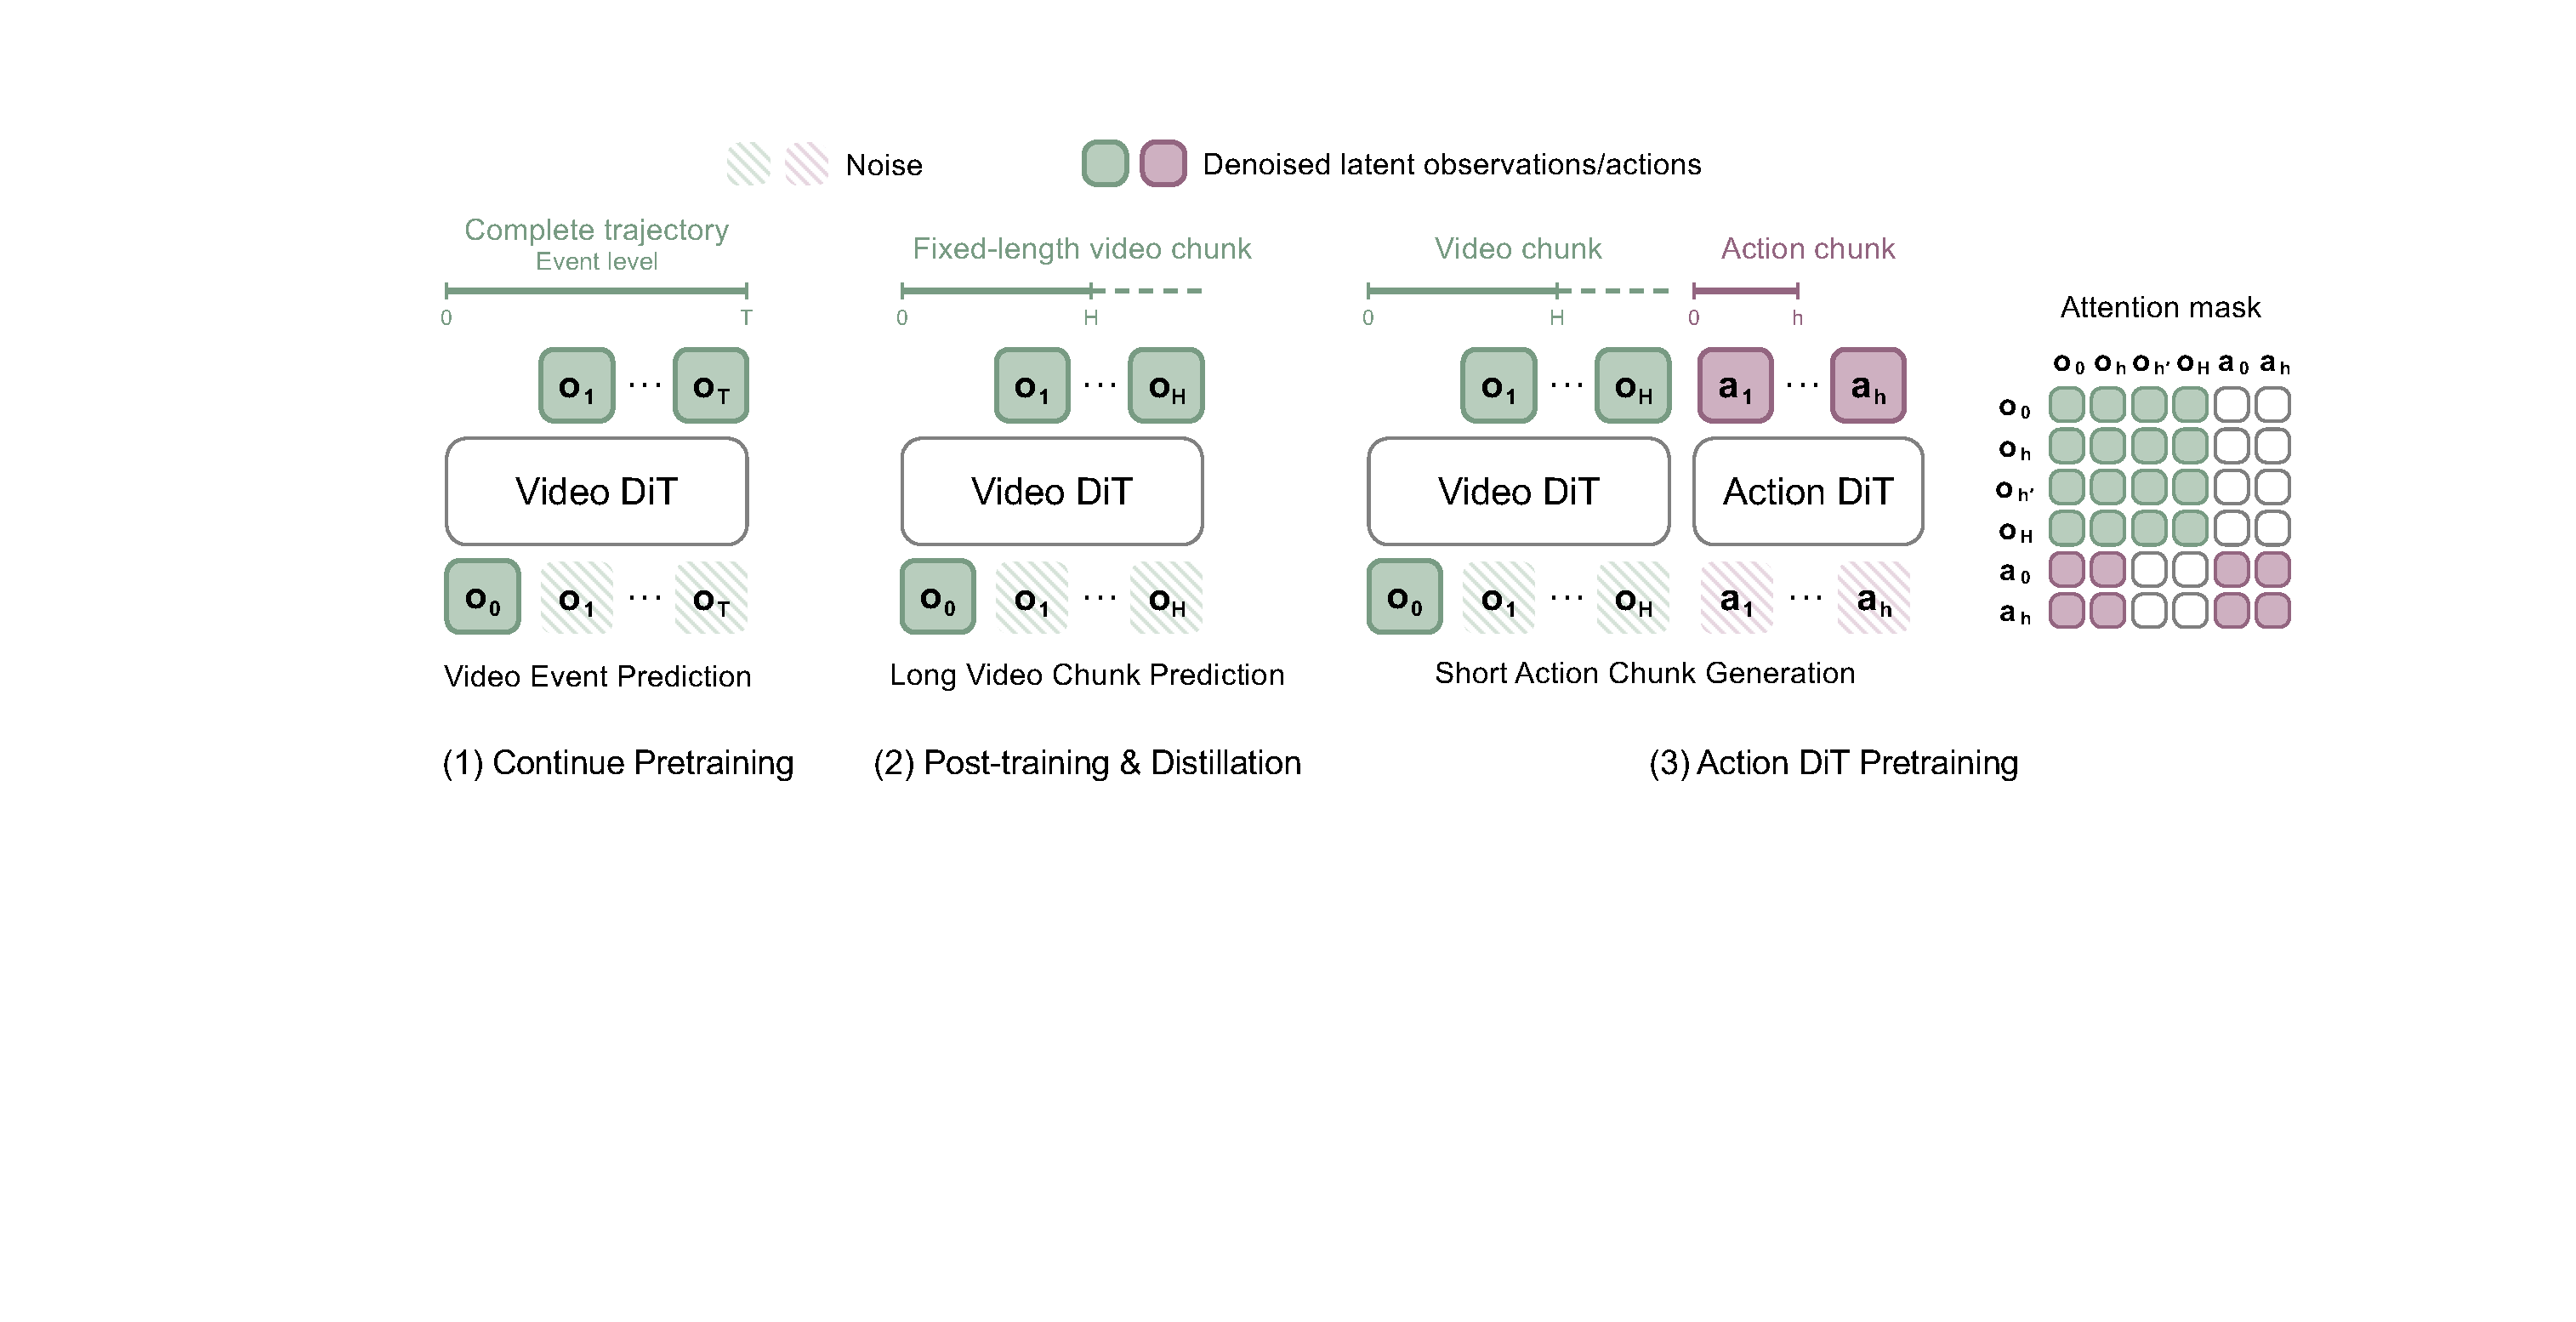
\includegraphics[width=0.95\linewidth]{figures/fig4_3.pdf}
    \caption{The VPP2 training pipeline is designed to maximize generalization. Stage 1 uses large-scale, event-level video pretraining to learn a generalizable video model for manipulation. Stage 2 post-trains and distills this model to predict long-horizon video chunks spanning 8 seconds in a single forward pass, taking approximately 0.1 seconds. Finally, Stage 3 trains an action expert to generate 2-second action chunks conditioned on the one-step video latents.}
    \label{fig:fig4}
\end{figure}

\medskip
\noindent
\textbf{Stage 2: Chunk-level Video Model Post-training.}
Event-level continued pre-training enables the model to generalize well to manipulation tasks.
However, sampling a fixed number of frames from events of different
durations produces variable temporal intervals between predicted
frames, complicating their alignment with downstream actions.
We therefore further post-train the model to predict a fixed-duration
future chunk, establishing a consistent temporal scale for
action learning. In experiments, we predict 2 seconds for human-hand manipulation and 8 seconds for robot manipulation.

Let $H$ denote the prediction horizon in seconds and $f$ the
dataset frame rate in frames per second (fps).
The nominal interval between sampled frames is
$\delta = fH/N$, measured in dataset frames.
For a chunk starting at frame $t$, the target video is
\begin{equation}
    \mathbf{y}_{\mathrm{chunk}}^{(t)}
    =
    \left( o_t,
        o_{t+\lfloor \delta \rfloor},
        o_{t+\lfloor 2\delta \rfloor},
        \ldots,
        o_{t+\lfloor N\delta \rfloor}
    \right),
\end{equation}
with conditioning inputs $c$ containing the observation $o_t$
and the corresponding subtask instruction.
The index $t+\lfloor fH \rfloor$ is capped at the final frame index $T$, and we optimize the same flow matching
objective in Eq.~\eqref{eq:video_fm}, with
$\mathbf{x}_1 = \mathcal{E}(\mathbf{y}_{\mathrm{chunk}}^{(t)})$.

\medskip
\noindent
\textbf{Stage 2: Consistency Distillation.}\label{consistency}
We distill the chunk-level video model for single-step generation~\citep{song2023consistency}
by enforcing consistent terminal predictions at adjacent flow times:
\begin{equation}
    \mathcal{L}_{\mathrm{CD}}
    =
    \mathbb{E}
    \left[
        \lambda(s,s')
        \left\|
            F_\theta(\mathbf{x}_s,s,c)
            -
            \operatorname{stopgrad}\left(
                F_{\bar{\theta}}(\widehat{\mathbf{x}}_{s'},s',c)
            \right)
        \right\|_2^2
    \right],
\end{equation}
where $0 \leq s < s' \leq 1$,
$\widehat{\mathbf{x}}_{s'}$ is obtained by integrating the frozen
teacher flow from $(\mathbf{x}_s,s)$ to $s'$, and
$\bar{\theta}$ denotes the EMA student parameters.
The student satisfies $F_\theta(\mathbf{x},1,c)=\mathbf{x}$.
To emphasize single-step generation, we sample $s'=1$ with
probability $0.5$;
otherwise, we sample $s'$ from the remaining flow times.
At inference, the video latent is generated in a single forward
pass as $F_\theta(\boldsymbol{\epsilon},0,c)$.



\subsection{Action Modeling}
\textbf{Stage 3: Action Pretraining across Datasets.}
After training a generalizable video model, we train the action expert on our processed bimanual datasets with unified workspace and end-effector coordinate systems. The action expert is a 0.9B-parameter diffusion transformer (DiT)~\citep{peebles2023scalable} with a standard MoT architecture. Since the action expert is newly initialized, we freeze the base parameters of the video DiT during the early stages of action training and adapt the video backbone using only LoRA~\citep{hu2022lora}. This strategy helps preserve the pretrained video representations while limiting disruption from action-training gradients.

\textbf{Inference Latency.}
We generate video efficiently by reducing the video input to \(17\times416 \times 240\) during post-training and distilling the video model for one-step generation, as described in Sec.~\ref{consistency}. With bfloat16 precision and torch.compile, the video model takes approximately 0.12 seconds. The action expert then generates an action chunk conditioned on the video latents using five denoising steps, taking approximately 0.1 seconds. The total latency per action chunk is therefore approximately 0.22 seconds.

% The original model processes videos at a spatiotemporal resolution of \(81 \times 832 \times 480\) and requires several seconds even for a single forward pass, making it impractical for real-time robotic systems. Rather than pursuing pixel-level fidelity, we prioritize reliable instruction following and informative future predictions that can effectively guide the action expert. Accordingly, we reduce the sequence length to 17 frames, comprising one observed frame and 16 predicted frames, and lower the spatial resolution to \(416 \times 240\). With this configuration, a forward pass takes approximately 0.12 seconds on a single GPU, satisfying the latency requirements of real-time policy inference.

\subsection{VLM for High-level Planning.}
\textbf{Sub-task Planning.} To tackle long-horizon tasks and handle ambiguous human instructions, we adopt a hierarchical architecture in which a VLM generates subtask plans~\citep{shi2025hi}. The VLM handles high-level reasoning, semantic understanding, and memory, allowing VPP2 to focus on mapping explicit instructions to trajectories. In practice, the VLM can be deployed locally or accessed through an API to a frontier model.

\textbf{Prompt Enhancement.}
VLM planning also generates detailed subtask descriptions that match the caption template used during training. Prior work on video generation likewise highlights the importance of detailed captions for generation quality~\citep{wan2025wan,yang2025cogvideox}.






% Requires: \usepackage{booktabs}
% \begin{table}[h]
%     \centering
%     \small
%     \setlength{\tabcolsep}{4pt}
%     \renewcommand{\arraystretch}{1.15}
%     \begin{tabularx}{\linewidth}{@{}llXr@{}}
%         \toprule
%         Data Type & Embodiment Type & Data Sources & Total Time \\
%         \midrule
%         \multirow{3}{*}{Robot}
%         & Single-arm
%         & OXE, RoboMIND, DROID, RH20T, Molmoact
%         & 3,624 h \\
%         & Dual-arm
%         & AgibotWorld-Beta, RoboCOIN, RDT, GM100, ABC-130k, Self-collected Aloha
%         & 10,307 h \\
%         & Mobile \& humanoid
%         & InternData-A1, Galaxea Open-World
%         & 868 h \\
%         \midrule
%         \multirow{2}{*}{Human}
%         & \multirow{2}{*}{Human hands}
%         & Open-source: EgoDex, Ego4D, Epic-Kitchen
%         & 4,599 h \\
%         & & Self-collected & $\approx10,000$h \\
%         \midrule
%         General Video
%         & Human hands
%         & Open-vid, Panda-70M
%         & --- \\
%         \bottomrule
%     \end{tabularx}
%     \caption{Placeholder Caption}
%     \label{table:video_source}
% \end{table}